%%
%% This is file `sample-sigconf.tex',
%% generated with the docstrip utility.
%%
%% The original source files were:
%%
%% samples.dtx  (with options: `all,proceedings,bibtex,sigconf')
%% 
%% IMPORTANT NOTICE:
%% 
%% For the copyright see the source file.
%% 
%% Any modified versions of this file must be renamed
%% with new filenames distinct from sample-sigconf.tex.
%% 
%% For distribution of the original source see the terms
%% for copying and modification in the file samples.dtx.
%% 
%% This generated file may be distributed as long as the
%% original source files, as listed above, are part of the
%% same distribution. (The sources need not necessarily be
%% in the same archive or directory.)
%%
%%
%% Commands for TeXCount
%TC:macro \cite [option:text,text]
%TC:macro \citep [option:text,text]
%TC:macro \citet [option:text,text]
%TC:envir table 0 1
%TC:envir table* 0 1
%TC:envir tabular [ignore] word
%TC:envir displaymath 0 word
%TC:envir math 0 word
%TC:envir comment 0 0
%%
%% The first command in your LaTeX source must be the \documentclass
%% command.
%%
%% For submission and review of your manuscript please change the
%% command to \documentclass[manuscript, screen, review]{acmart}.
%%
%% When submitting camera ready or to TAPS, please change the command
%% to \documentclass[sigconf]{acmart} or whichever template is required
%% for your publication.
%%
%%
\PassOptionsToPackage{expansion=false}{microtype}
\documentclass[sigconf, nonacm]{acmart}
\usepackage{tabularx}
\usepackage{ragged2e}
\newcolumntype{L}{>{\RaggedRight\arraybackslash}X}
\usepackage{booktabs}
\usepackage{float}
\usepackage{tikz}
\usetikzlibrary{shapes.geometric, arrows.meta, positioning, calc, fit, backgrounds}

\tikzset{
    block/.style={rectangle, draw, fill=blue!5, text width=6em, text centered, rounded corners, minimum height=3em, font=\small},
    subblock/.style={rectangle, draw, fill=gray!10, text width=5em, text centered, rounded corners, minimum height=2.5em, font=\footnotesize},
    io/.style={trapezium, trapezium left angle=70, trapezium right angle=110, draw, fill=green!5, text width=4em, text centered, minimum height=2em, font=\small},
    cloud/.style={draw, ellipse, fill=red!5, text width=6em, text centered, minimum height=3em, font=\small},
    decision/.style={diamond, draw, fill=yellow!5, text width=4.5em, text centered, inner sep=0pt, font=\footnotesize},
    arrow/.style={thick, ->, >=stealth},
    phase/.style={rectangle, draw, dashed, inner sep=0.3cm, font=\bfseries\small}
}
%%
%% \BibTeX command to typeset BibTeX logo in the docs
\AtBeginDocument{%
  \providecommand\BibTeX{{%
    Bib\TeX}}}

%% Rights management information.  This information is sent to you
%% when you complete the rights form.  These commands have SAMPLE
%% values in them; it is your responsibility as an author to replace
%% the commands and values with those provided to you when you
%% complete the rights form.
\setcopyright{acmlicensed}
\copyrightyear{2018}
\acmYear{2018}
\acmDOI{XXXXXXX.XXXXXXX}
%% These commands are for a PROCEEDINGS abstract or paper.
% \acmConference[Conference acronym 'XX]{Make sure to enter the correct
%   conference title from your rights confirmation email}{June 03--05,
%   2018}{Woodstock, NY}
%%
%%  Uncomment \acmBooktitle if the title of the proceedings is different
%%  from ``Proceedings of ...''!
%%
%%\acmBooktitle{Woodstock '18: ACM Symposium on Neural Gaze Detection,
%%  June 03--05, 2018, Woodstock, NY}
\acmISBN{978-1-4503-XXXX-X/2018/06}


%%
%% Submission ID.
%% Use this when submitting an article to a sponsored event. You'll
%% receive a unique submission ID from the organizers
%% of the event, and this ID should be used as the parameter to this command.
%%\acmSubmissionID{123-A56-BU3}

%%
%% For managing citations, it is recommended to use bibliography
%% files in BibTeX format.
%%
%% You can then either use BibTeX with the ACM-Reference-Format style,
%% or BibLaTeX with the acmnumeric or acmauthoryear sytles, that include
%% support for advanced citation of software artefact from the
%% biblatex-software package, also separately available on CTAN.
%%
%% Look at the sample-*-biblatex.tex files for templates showcasing
%% the biblatex styles.
%%

%%
%% The majority of ACM publications use numbered citations and
%% references.  The command \citestyle{authoryear} switches to the
%% "author year" style.
%%
%% If you are preparing content for an event
%% sponsored by ACM SIGGRAPH, you must use the "author year" style of
%% citations and references.
%% Uncommenting
%% the next command will enable that style.
%%\citestyle{acmauthoryear}
\usepackage{pgfplots}
\pgfplotsset{compat=1.18}

%%
%% end of the preamble, start of the body of the document source.
\begin{document}

%%
%% The "title" command has an optional parameter,
%% allowing the author to define a "short title" to be used in page headers.
\title{Revolutionizing Urban Mobility: Design and Evaluation of a Contactless (NFC/HCE) Payment System for Seamless Public Transit Fare Transactions. }

%%
%% The "author" command and its associated commands are used to define
%% the authors and their affiliations.
%% Of note is the shared affiliation of the first two authors, and the
%% "authornote" and "authornotemark" commands
%% used to denote shared contribution to the research.
\author{Prashant Adhikari}
\authornote{Corresponding author.}
\email{prashant_adhikari_a25@sunway.edu.np}
\orcid{0009-0008-6960-7907}
\affiliation{%
  \institution{Sunway College Kathmandu}
  \city{Kathmandu}
  \state{Bagmati}
  \country{Nepal}
}

\author{Maladeep Upadhyaya}
\email{maladeep@sunway.edu.np}

\affiliation{%
  \institution{Sunway College Kathmandu}
  \city{Kathmandu}
  \state{Bagmati}
  \country{Nepal}}

\author{Supriya Khadka}
\email{supriya@sunway.edu.np}
\affiliation{%
  \institution{Sunway College Kathmandu}
  \city{Kathmandu}
  \state{Bagmati}
  \country{Nepal}}

%%
%% By default, the full list of authors will be used in the page
%% headers. Often, this list is too long, and will overlap
%% other information printed in the page headers. This command allows
%% the author to define a more concise list
%% of authors' names for this purpose.
\renewcommand{\shortauthors}{Prashant A.}

%%
%% The abstract is a short summary of the work to be presented in the
%% article.
\begin{abstract}
Commuting in Nepal’s busiest cities, like Kathmandu and Pokhara, is often a source of daily frustration, largely because our fare systems are still stuck in a cash-only era. While many hoped QR code-based payments with Esewa or Khalti would digitize the payment infrastructure in public transportation, they’ve proven to be a headache in a moving bus, as they’re just too slow to scan and completely fall apart the moment the mobile signal drops. Our work details the development of TransitPay, a system built to bypass these hurdles using Near Field Communication (NFC) and Host Card Emulation (HCE). By combining simple, affordable hardware like the ESP8266 and PN532 alongside GPS modules such as the NEO6M with a custom Android app, we’ve created a tap-and-go setup that works for both smartphones and physical transit cards. To make sure the system stays reliable even in areas with “patchy” internet, we designed a local queuing method, which allows the hardware to process payments offline and then sync everything to the cloud once the vehicle is back in range. Furthermore, the point-of-sale-only internet requirement also solves major issues of internet unavailability in users' smartphones. While a typical QR transaction in Nepal drags on for 35 seconds and can take over a minute when the connection is poor, TransitPay hits a best-case speed of just 1.5 to 2.5 seconds, making a significant decrement in the transaction time by almost 91.7 percent. Even in the worst case, the process wraps up in 10 seconds, still making it efficient by decreasing the time constraint by almost 71.4 percent. These results prove that moving toward an NFC-based infrastructure isn’t just about new tech; it’s about making public transport faster, fairer, and finally fit for the digital age.

\end{abstract}

%%
%% The code below is generated by the tool at http://dl.acm.org/ccs.cfm.
%% Please copy and paste the code instead of the example below.
%%


%%
%% Keywords. The author(s) should pick words that accurately describe
%% the work being presented. Separate the keywords with commas.
\keywords{Fintech, Public transportation, Near-Field-Technologies, Host Card Emulation, Internet of Things}
%% A "teaser" image appears between the author and affiliation
%% information and the body of the document, and typically spans the
%% page.

% \received{20 February 2007}
% \received[revised]{12 March 2009}
% \received[accepted]{5 June 2009}

%%
%% This command processes the author and affiliation and title
%% information and builds the first part of the formatted document.
\maketitle

\section{Introduction}
Urban mobility plays a crucial role in the social and economic development of developing countries like Nepal. Rapid urbanization, especially in cities such as Kathmandu, Lalitpur, and Pokhara, has led to a significant increase in the use of public transportation systems, including buses, microbuses, and tempo services. However, Nepal’s public transit fare collection system is still largely dependent on cash-based transactions, which often result in inefficiencies such as long boarding times, fare disputes, revenue leakage, lack of transparency, and inconvenience for both passengers and transport operators.

With the growing penetration of smartphones, digital wallets, and contactless technologies in Nepal, there is a strong opportunity to modernize public transportation payment systems. Technologies such as Near Field Communication (NFC) and Host Card Emulation (HCE) enable secure, fast, and contactless fare payments using smartphones or smart cards without the need for physical cash. Several countries have successfully implemented contactless fare systems to improve passenger convenience, operational efficiency, and financial accountability. However, Nepal has been slow in adopting such technologies in its public transport sector due to infrastructural, regulatory, and awareness-related challenges.

The Government of Nepal and private financial institutions have recently promoted digital payment platforms as part of the national digital economy initiative. Despite this progress, the integration of digital payment systems into public transit remains limited and fragmented. A unified, contactless fare payment system could significantly enhance the urban transit experience by reducing boarding time, minimizing human error, improving data collection for transit planning, and supporting cashless economic policies.


\section{Literature Review}
Public transportation in Nepal remains heavily reliant on fragmented, cash-based fare collection. This manual system is plagued by operational inefficiencies, including widespread fare evasion and a lack of pricing consistency~\cite{shreya2025nepal}. Furthermore, the absence of digital transaction records deprives transport authorities of the real-time ridership data necessary for effective urban planning and service optimization (Coseco Services, n.d.) \cite{coseco_services_working_nodate}. As urban centers like Kathmandu grow, the need for a seamless, transparent, and data-driven payment ecosystem becomes critical.

\subsection{The introduction of NFC in the tech world}

Near Field Communication (NFC) originated from the groundwork of Radio-Frequency Identification (RFID), evolving into a specialized protocol for secure, short-range interaction. The modern tech world saw the official birth of this standard through a 2002 collaboration between Sony and Philips, which eventually led to the 2004 establishment of the NFC Forum~\cite{kaiser2017nfc}. This standardization was essential for defining the 13.56 MHz frequency and the ISO/IEC 18092 standards that allow for seamless data exchange between active and passive devices~\cite{singh2020near}. By limiting communication to a range of approximately 4 cm, the technology ensures that data transfer is both intentional and secure, moving NFC from niche industrial use to a consumer-facing interface.

The integration of NFC into mobile hardware transformed smartphones into digital hubs, moving beyond simple communication to facilitate a "cashless society." While early devices like the Nokia 6131 pioneered the hardware, the momentum shifted significantly with the launch of major digital wallets, which utilized the device's magnetic field induction principles for secure transactions~\cite{nikam2017near}. This era introduced the ability to store encrypted tokens on mobile devices, allowing users to replace physical cards with a single tap. As adoption grew, consumer behavior began to shift based on increased trust and self-efficacy in these mobile payment models, cementing NFC as a global retail standard~\cite{aloufi2025investigating}.

Today, NFC has matured into a ubiquitous technology that underpins the modern IoT (Internet of Things) ecosystem and public infrastructure. Current industry roadmaps highlight an evolution toward "multi-purpose taps" and increased range, expanding its utility into smart home integration, automotive digital keys, and identity verification~\cite{staff2023nfc}. Recent studies indicate a "device-first" approach where consumers increasingly rely on NFC for everything from public transit to authenticated supply chain logistics~\cite{nfcforum2024device}. This ongoing development ensures that the technology remains a vital driver of "tap-and-go" convenience across various sectors of the digital economy.

\subsection{The early use of NFC}

The early use of Near Field Communication (NFC) was defined by experimental pilot programs and the first wave of hardware integration that sought to prove the concept of a "mobile wallet." While the technology was standardized in 2004, its practical debut occurred in 2006 with the release of the Nokia 6131 NFC, the first mass-market phone to feature a built-in NFC chip~\cite{nokia2007nfc}. Early use cases were not limited to payments; they focused on the "just touch" philosophy to simplify complex tasks. In 2007, a landmark trial in London partnering Nokia, Barclays, and Transport for London which allowed participants to use their mobile devices as both a prepaid Visa card and an Oyster transit card~\cite{kaiser2017nfc}. This period demonstrated that NFC could successfully merge financial services with public infrastructure through a single physical gesture.

Before it became a standard feature in every smartphone, early NFC applications explored the "Reader/Writer" and "Peer-to-Peer" modes to bridge the gap between physical objects and digital data. In 2006, some of the first commercial applications included using NFC-enabled stickers or "tags" in libraries to assist disabled patrons in accessing resources~\cite{lathiya2021near}. By 2010, the telecommunications sector had launched over 100 pilot projects worldwide, testing everything from "Smart Posters" that triggered web links when tapped to hotel room entry systems~\cite{tardi2023near}. These early implementations were critical for identifying the technical requirements for magnetic field induction and active/passive communication, ensuring that the devices could operate reliably within the strict 4 cm range required for security~\cite{singh2020near}

The transition from experimental trials to mainstream utility was marked by the launch of the Samsung Nexus S in 2010, the first Android device to fully integrate NFC, which paved the way for Google Wallet in 2011~\cite{tragging2023history}. This era saw the introduction of programmable tags, such as Samsung TecTiles (2012) and Sony’s Xperia SmartTags, which allowed users to automate phone settings, like turning on an alarm or silencing a ringer, by tapping their device against a physical sticker~\cite{lathiya2021near}. These early consumer-led uses were essential for socializing the "tap" gesture among the public, moving the technology away from its industrial RFID roots and toward the intuitive, frictionless experience that defines modern digital interaction.


\subsection{Host Card Emulation and early implementation}

The early era of Near Field Communication (NFC) was defined by a hardware-centric model known as the Secure Element (SE), which created a period of significant market fragmentation often referred to as the "Secure Element wars." In this framework, sensitive payment credentials were required to be stored in a physical, tamper-resistant microchip, which could reside in the phone's SIM card, an embedded chip (eSE), or a microSD card~\cite{lepojevic2014implementing}. This early implementation forced service providers, such as banks, to negotiate complex commercial agreements with Mobile Network Operators (MNOs) to gain access to the "keys" of the SIM-based SE~\cite{thales2023host}. Consequently, mass adoption was stifled by these gatekeepers, as carriers often blocked competing digital wallets to promote their own proprietary services, such as the ill-fated Softcard (formerly Isis) venture in the United States.

A transformative shift occurred in 2013 with the introduction of Host Card Emulation (HCE) in Android 4.4 (KitKat). Developed to bypass the reliance on physical hardware and carrier control, HCE allowed the smartphone's main operating system to emulate a smart card using software rather than a dedicated hardware chip~\cite{nikam2017near}. This architecture routes the NFC protocol directly to the host CPU, enabling any application to act as a virtual contactless card by leveraging "cloud-based SE" models. By moving the security layer from the physical device to the cloud, HCE effectively "democratized" NFC development, allowing banks and transit authorities to launch mobile wallets independently of mobile carriers~\cite{prakash2015host}.

While HCE provided the flexibility needed for global scaling, it introduced new security challenges since the host operating system is generally more vulnerable to software attacks than a hardware-isolated SE. To mitigate these risks, modern HCE implementations rely heavily on tokenization and Limited Use Keys (LUKs), which ensure that even if a transaction's data is intercepted, it cannot be reused for subsequent payments~\cite{crowe2016understanding}. Today, the industry has largely settled on a hybrid approach; while Apple Pay continues to use a hardware-embedded Secure Element for maximum security, most Android-based wallets use HCE to ensure compatibility across a vast range of hardware, demonstrating how software-based emulation saved NFC from a future of carrier-controlled silos~\cite{whitepaperhce}.


\subsubsection{Regional Adoption Trends of NFC based payments}

The adoption of NFC payments varies significantly by geography, driven by local infrastructure and regulatory support:


\begin{itemize}
    \item \textbf{Europe:} Leads in retail penetration, with nearly 90\% of all retail transactions being contactless in 2026~\cite{ejimone2025contactless}. Countries such as the UK and Ireland report that over 60\% of these transactions are made specifically via smartphones rather than plastic cards.
    
    \item \textbf{Asia--Pacific:} Remains the largest market by transaction volume, contributing roughly 40\% of all global NFC transactions~\cite{dey2025nfc}. While QR codes historically dominated in China and India, NFC is surging in Southeast Asia, with countries like the Philippines, Thailand, and Vietnam projected to reach 75\% digital wallet penetration by late 2026~\cite{juniper2022digital}.
    
    \item \textbf{North America:} Accounts for roughly 36\% of global demand share, dominated by the ``Big Three'' OEM wallets: Apple Pay, Google Pay, and Samsung Pay. The U.S.\ has seen a rapid shift among Gen~Z and Millennials, with 70\% of these demographics using NFC as their primary shopping method.
\end{itemize}


\subsubsection{Emerging Use Cases and Infrastructure}


The current market is moving beyond simple retail transactions toward integrated ``Smart City'' ecosystems. A key trend in 2026 is the rise of \textit{SoftPOS} (Software Point-of-Sale), which allows merchants to turn any standard NFC-enabled smartphone into a payment terminal without additional hardware---a technology that saw a 234\% increase in transactions in certain markets over the last year~\cite{valero2025rise}.

Furthermore, the introduction of \textit{Multi-Purpose Taps} allows a single gesture to process a payment, apply a loyalty discount, and issue a digital receipt simultaneously. This integration is particularly prominent in public transit and the circular economy, where ``regenerative payment loops'' incentivize sustainable consumer choices through microtransactions~\cite{hyman2025future}.

\subsection{Use of NFC and RFID in Transportation Management}

In Nepal, the adoption of NFC and RFID in transportation has shifted from experimental pilot phases to becoming mandatory national infrastructure. While RFID is primarily used for long-range vehicle identification and tracking, NFC is utilized for short-range passenger interactions and transit payments.

\subsubsection{RFID: National Vehicle Tracking and Embossed Plates}

The most significant implementation of RFID in Nepal is the Electronic Vehicle Number Plate (EVNP) system, commonly known as embossed number plates.

\begin{itemize}
    \item \textbf{Mandatory Integration:} As of September 17, 2025, the Department of Transport Management (DoTM) made embossed number plates mandatory for all new registrations, ownership transfers, and renewals. The decision was later withdrawn due to widespread public backlash~\cite{khatri2025embossed}.
    
    \item \textbf{The RFID Chip:} Each plate contains a high-security RFID microchip that stores the vehicle’s unique registration data, engine number, and owner details~\cite{omoda2025embossed}.
    
    \item \textbf{Security \& Infrastructure:} The government has initiated the construction of 100 RFID gates across the country, with operational gates already installed at key entry points such as Nagdhunga and Nagarjun. These gates automatically scan vehicles as they pass, enabling real-time traffic monitoring and assisting law enforcement in tracking stolen vehicles without requiring physical stops~\cite{khatri2025embossed}.
\end{itemize}


\subsubsection{NFC: Smart Ticketing and the "Yatra Card"}

In the public transit sector, NFC technology is used to facilitate contactless payments, aiming to reduce "revenue leakage," where conductors might not report full cash earnings.

\begin{itemize}
    \item \textbf{Sajha Yatayat and Smart Cards:}  Sajha Yatayat pioneered the Smart Travel Card system in Kathmandu. Passengers tap an NFC card on readers located at the bus doors upon entry and exit. The system automatically calculates the fare based on the distance traveled~\cite{shreya2025nepal}.
    
    \item \textbf{The Yatra Card:} Fintech International’s Yatra Card is a prominent NFC-enabled smart card in Nepal. It allows commuters to store up to Rs. 25,000 and can be topped up via mobile wallets or bank accounts. It is designed specifically for a "tap-in, tap-out" experience, providing a printed or digital receipt of the fare deducted~\cite{fintech2023yatra}.
    
    \item \textbf{Digital Address System (DAS):} In 2025, the Kathmandu Metropolitan City (KMC) also launched an NFC-based digital address system in Ward No. 26. While not directly for "moving" transport, these plates are placed on houses near transport hubs (like the New Bus Park) to provide digital location data for logistics and emergency services~\cite{bhatta2025kathmandu}.
\end{itemize}

\subsection{Existing potential Fintech System in Transportation and gaps}

The digital payment landscape in Nepal has seen a "mobile-first" explosion, with over a 23-fold increase in Payment Service Provider (PSP) agents by 2025 (Kanya Journal, 2025). However, the application of this growth to urban transit remains inefficient.

\subsubsection{Direct Comparison of Transit Modalities}

The table below outlines the technological differences between current systems and the requirements for a seamless transit ecosystem.


\begin{table}[H]
\centering
\caption{Feature Comparison Between Traditional QR and NFC Enabled Cards}
\begin{tabular}{lll}
\toprule
\textbf{Feature} & \textbf{Esewa/Khalti QR} & \textbf{Smart Cards} \\
\midrule
Transaction Speed & Slow (15--30 sec) & Fast ($<$ 5s) \\
User Onboarding   & Digital (App) & Physical (Card) \\
Security          & Low (Raw data) & High (Secured) \\
Hardware Cost     & Low (QR prints) & High (POS) \\
\bottomrule
\end{tabular}
\end{table}

\subsubsection{Identified Gaps in Nepal's Ecosystem} \mbox{} \\

\textbf{The Interoperability Gap:} Existing smart cards are "Closed-Loop," meaning a Sajha card cannot be used on a private microbus. While the National Payment Switch (NPS) has integrated retail wallets, it lacks a standardized "Transit API" for cross-operator fare settlement~\cite{nrb2024payment}.

\begin{itemize}
    \item \textbf{The "Boarding Latency" Gap:} Research shows that QR code adoption in Kathmandu is high for retail but fails in transit because "Transaction Failure" is the biggest concern for mobile users (ResearchGate, 2024). Manual QR scanning takes over 10 seconds, causing "stacking" at bus doors, whereas NFC-based systems reduce this to milliseconds~\cite{harnaningrum2024comparison}.

    \item \textbf{The Information Deficit Gap:} Commuters in Kathmandu express a "high desirability" for digital help because they cannot track routes or fares in real-time (St. Xavier's Transit Survey, 2023). Existing fintech only handles the payment but fails to provide the ridership data needed for navigation~\cite{ghimire2023issues}.

    \item \textbf{The Resilience/Infrastructure Gap:} Nepal’s "patchy broadband" and weak last-mile connectivity limit real-time cloud payments (Digital Economy \& Financial Innovation Report, 2025). Current systems lack the "Offline Data Queuing" necessary for a moving vehicle crossing network blind spots~\cite{kharel2023digital}.
\end{itemize}

\section{Methodology}

In this section, we will outline the methodology we approached to design and develop our proposed system that works as the payment service provider for the public transit in metro cities of Nepal.  While various engineering design methodologies exist, ranging from the software-centric Agile framework used for rapid application iteration to the hardware-focused V-Model for protocol verification, this research adopts a Systems Engineering Design Methodology. This approach is specifically chosen to harmonize the multi-layered complexity of the TransitPay ecosystem, ensuring seamless integration between the IoT hardware (ESP8266/PN532), the HCE-enabled React Native mobile client, and the MongoDB-backed Node.js server. This section will be divided into seven distinct parts: system design, user flow pipeline, and cost breakdown.

\subsection{System Design}


The system design and architecture of the proposed system is secure with the communication of the NFC entity and the point of sale, with the POS sending APDU challenges to the NFC entity, and after the entity solves the APDU challenges, it sends the encrypted data using the entity’s unique private key; afterwards, the POS decrypts the data using the public key embedded in it, and then the communication between the NFC entity and the POS is successful. 


\begin{figure*}[t]
  \centering
  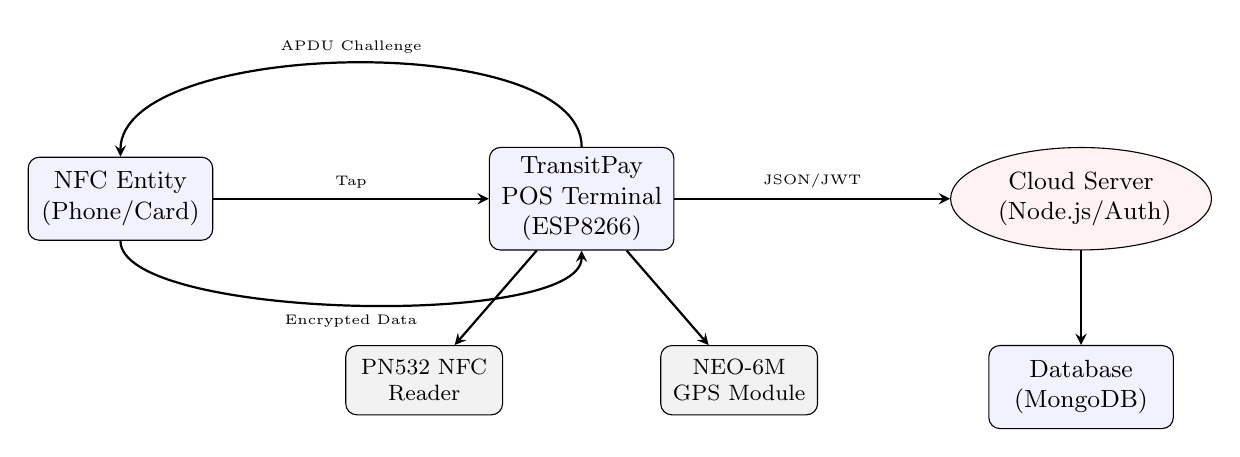
\begin{tikzpicture}[node distance=3.5cm]
    % Central POS
    \node (pos) [block] {TransitPay POS Terminal (ESP8266)};
    
    % Peripherals
    \node (entity) [block, left=of pos] {NFC Entity (Phone/Card)};
    \node (pn532) [subblock, below=1.2cm of pos, xshift=-2cm] {PN532 NFC Reader};
    \node (neo6m) [subblock, below=1.2cm of pos, xshift=2cm] {NEO-6M GPS Module};
    
    % Infrastructure
    \node (server) [cloud, right=of pos] {Cloud Server (Node.js/Auth)};
    \node (db) [block, below=1.2cm of server] {Database (MongoDB)};

    % Primary Flow
    \draw [arrow] (entity) -- node[above, font=\tiny] {Tap} (pos);
    \draw [arrow] (pos) -- (pn532);
    \draw [arrow] (pos) -- (neo6m);
    \draw [arrow] (pos) -- node[above, font=\tiny] {JSON/JWT} (server);
    \draw [arrow] (server) -- (db);
    
    % APDU Handshake (Curved to avoid overlapping)
    \draw [arrow] (pos.north) .. controls +(up:1.5cm) and +(up:1.5cm) .. node[above, font=\tiny] {APDU Challenge} (entity.north);
    \draw [arrow] (entity.south) .. controls +(down:1cm) and +(down:1cm) .. node[below, font=\tiny] {Encrypted Data} (pos.south);
  \end{tikzpicture}
  \caption{Redesigned system block diagram showing the interaction between hardware components and cloud infrastructure (Two-column layout).}
  \label{fig:system_block}
  \Description{System block diagram of transitpay.}
\end{figure*}

\subsubsection{NFC Trigger} \mbox{} \\

Near Field Technologies is proven to be effective for communication over a very small distance, making the communication between master and slave very secure. According to the NFC Forum, many NFC cards are manufactured, but one of the most secure cards among them is the DESFire EV3 card that utilizes AES-128, with options for 3DES, ensuring data confidentiality.~\cite{mifaredesfireev3}. The card and reader verify each other before data exchange, preventing unauthorized communication.~\cite{hidmifare}. 

% \begin{figure}
%     \centering
%     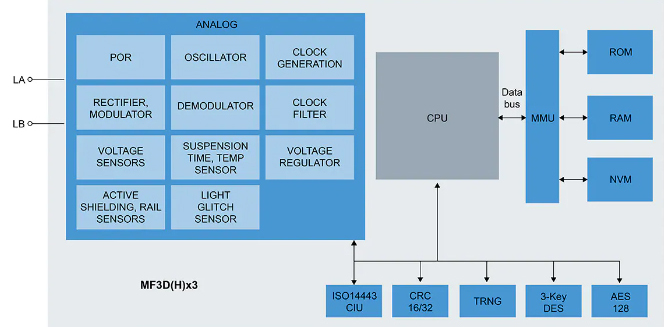
\includegraphics[width=1\linewidth]{MIFARE-DESFire-EV3.jpg}
%     \caption{DESFire EV3 block diagram}
%     \label{fig:mifare_desfire}
% \end{figure}

However, as the technologies evolve, our smartphones are also able to emulate themselves as an NFC card using Host Card Emulation (HCE)~\cite{hceoverview}. This system is explicitly tested using an Android phone. The TransitPay application, built using React Native, used APDU commands to communicate with the Payment Operating System. The application was tested using the AID number: D2760000850101. The KHostApduServices.kt and MainApplication.kt communicate with the IoT-embedded point of sale (POS) terminal.


\subsubsection{Point Of Sale Terminal} \mbox{} \\

The Point of Sale (POS) of the TransitPay ecosystem includes different Internet of Things modules such as a microcontroller, an NFC reader, a GPS module, and a local storage module.

During the test, ESP8266 is used as the main microprocessor module. The programming is done entirely in C++ inside the Arduino Integrated Development Environment. The ESP8266 (NodeMCU) development kit is considered the microprocessor module in this system because the ESP8266 (NodeMCU), serving as the main microcontroller for the TransitPay Point of Sale, is chosen because it is inexpensive, small in form factor, meets standards as a low-power processor, and has built-in Wi-Fi capabilities. It contains the required computational resources to manage NFC reader communications, perform fare validation, maintain local data storage of transactions, and periodically communicate and synchronize with the main server/backend.~\cite{esp8266soc}.
After a successful communication with an NFC card or an emulated card, the microcontroller communicates with the NEO6M GPS module for the extraction of the longitude and the latitude of the current location. The NEO-6M GPS module is chosen due to its high accuracy, reliability, low power consumption, and ease of integration with microcontroller-based systems. It provides real-time latitude and longitude data with good positional accuracy, which is essential for location-based authentication and transaction logging in NFC-enabled systems~\cite{gpsneo6m}. 

One of the key advantages of the NEO-6M is its UART-based serial communication, which allows seamless interfacing with controllers such as ESP8266, ESP32, Arduino, and STM32 without complex protocols. The module supports the standard NMEA output format, making data parsing straightforward and lightweight, which is ideal for embedded and IoT applications with limited resources~\cite{gpsneo6m}.

% \begin{figure}
%     \centering
%     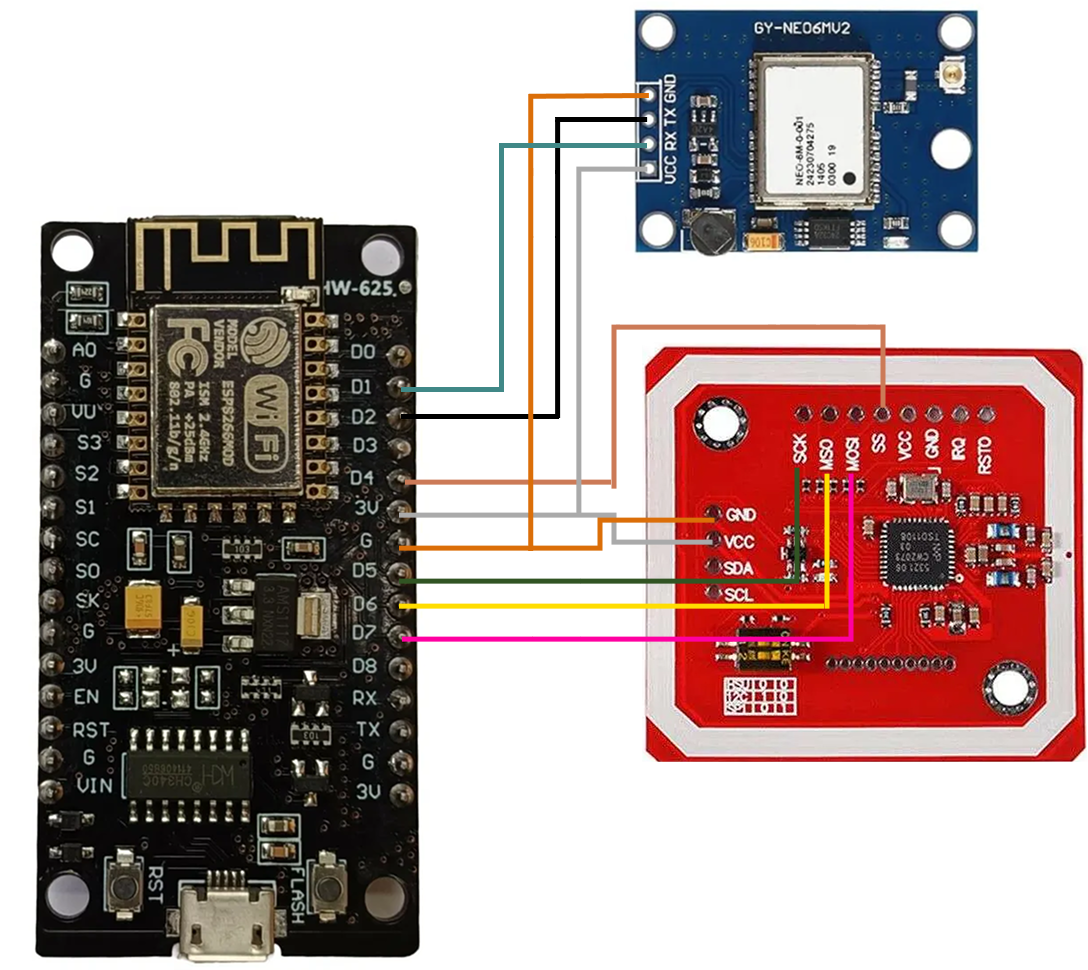
\includegraphics[width=1\linewidth]{IOT_components_wiring.png}
%     \caption{Illustration of connection of NodeMCU with PN532 and NEO-6M on SPI communication and UART communication respectively}
%     \label{fig:iot_components}
% \end{figure}

\subsubsection{Architectural Framework of the server}  \mbox{} \\

The TransitPay platform, a digital payment and transportation management solution, is powered by a strong backend system called TransitPay Server. It offers a full range of APIs for handling wallets, users, transactions, and the logistics of public transportation. It is the main hub for handling bus trips, processing NFC-based payments, and liaising with different organizational entities. It was designed with scalability and security in mind. Utilizing a cutting-edge Node.js and Express architecture, the system easily integrates with MongoDB to store persistent data.

To provide safe and precise permission management across various user roles, including administrators, ward officers, and commuters, it has an advanced Role-Based Access Control (RBAC) system. The backend also includes strong security features like rate limiting and JWT-based authentication, as well as real-time capabilities via Socket.io. This backend, which was created to support the TransitPay ecosystem, makes complicated processes like trip tracking, wallet top-ups, and card requests easier. Additionally, it ensures high availability and simplicity of integration for frontend applications and external services by offering health monitoring and a centralized entry point for multiple services.

The comprehensive details about how the fare are calculated in this system is described on a dedicated section "Fare Fare Model".

\subsubsection{The Fair Fare Model (FFM)}

The TransitPay system implements a Fair Fare Model to address the inefficiencies of fixed flat-fares, which often result in passengers overpaying for short-distance travel. This model utilizes an automated location-based mechanism to ensure that commuters are billed only for the specific stops traveled.

\textbf{Operational Mechanism}
The core logic of the model relies on a three-step transaction pipeline integrated with the vehicle's onboard IoT hardware:

\begin{enumerate}
    \item \textbf{Tap-In:} Upon boarding, the passenger taps their smartphone against the PN532 NFC module. The NEO-6M GPS module simultaneously logs the geographic coordinates of the boarding stop.
    \item \textbf{Tap-Out:} When the passenger reaches their destination and taps out, the system captures the alighting stop coordinates.
    \item \textbf{Lookup and Deduction:} The system matches the coordinate pair against a pre-loaded stop database on the ESP8266 microcontroller. The corresponding fare is retrieved from a fixed matrix and deducted instantly, requiring no manual calculation.
\end{enumerate}

\textbf{Fare Matrix Implementation}
The billing is governed by the Department of Transport Management (DoTM) guidelines. A representative sample of the Kathmandu Transit Fare Matrix (Fixed Rate) is detailed below:

\begin{table}[H]
  \centering
  \caption{Example of the fixed stop-based fare matrix}
  \label{tab:fare_matrix}
  \begin{tabular}{lccc}
    \toprule
    \textbf{From / To} & \textbf{Ratnapark} & \textbf{Lagankhel} & \textbf{Kalanki}\\
    \midrule
    \textbf{Ratnapark} & — & Rs. 30 & Rs. 35 \\
    \textbf{Lagankhel} & Rs. 30 & — & Rs. 25 \\
    \textbf{Kalanki}   & Rs. 35 & Rs. 25 & — \\
    \bottomrule
   \end{tabular}
\end{table}

By automating this process, the model eliminates revenue leakage and provides a scalable, low-cost path to digitizing transit fares.

\begin{figure*}[t]
\centering
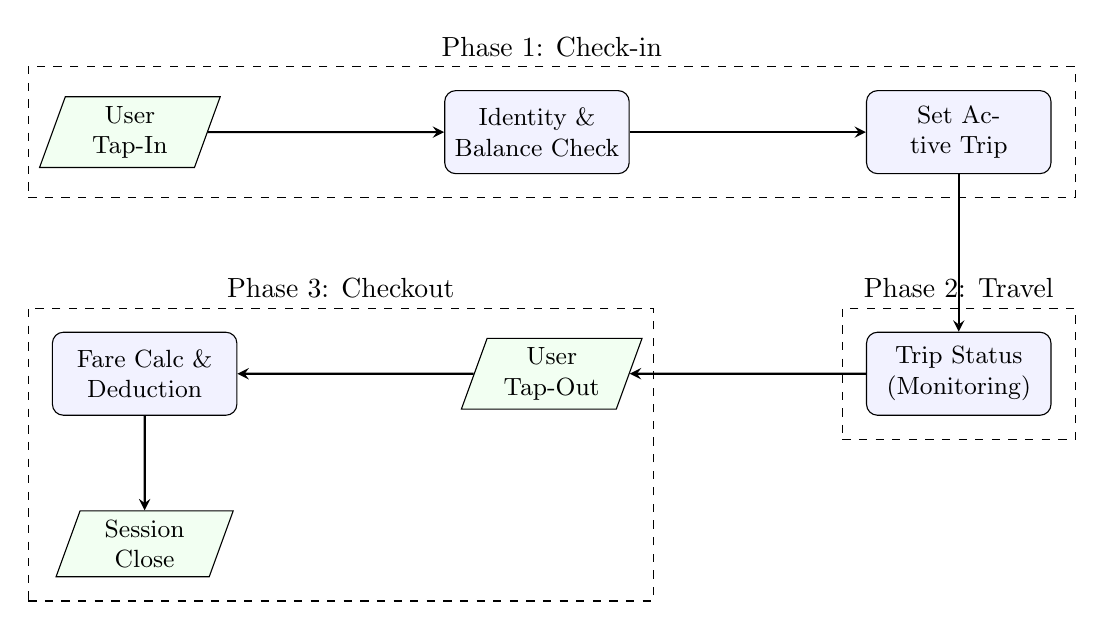
\begin{tikzpicture}[node distance=2cm and 3cm]
  % Nodes
  \node (tap) [io] {User Tap-In};
  \node (auth) [block, right=of tap] {Identity \& Balance Check};
  \node (active) [block, right=of auth] {Set Active Trip};
  
  \node (trip) [block, below=2cm of active] {Trip Status (Monitoring)};
  
  \node (exit) [io, left=of trip] {User Tap-Out};
  \node (fare) [block, left=of exit] {Fare Calc \& Deduction};
  \node (close) [io, below=1.2cm of fare] {Session Close};

  % Paths
  \draw [arrow] (tap) -- (auth);
  \draw [arrow] (auth) -- (active);
  \draw [arrow] (active) -- (trip);
  \draw [arrow] (trip) -- (exit);
  \draw [arrow] (exit) -- (fare);
  \draw [arrow] (fare) -- (close);

  % Phase Groupings (Block Structure)
  \begin{scope}[on background layer]
    \node[phase, fit=(tap)(auth)(active), label=above:Phase 1: Check-in] (p1) {};
    \node[phase, fit=(trip), label=above:Phase 2: Travel] (p2) {};
    \node[phase, fit=(exit)(fare)(close), label=above:Phase 3: Checkout] (p3) {};
  \end{scope}

\end{tikzpicture}
\caption{User flow block diagram organized by functional phases to ensure readability and logical grouping (Two-column layout).}
\label{fig:user_flow}
\end{figure*}

\subsection{Data collection and problem classification}
This section describes the analytical approach and procedures adopted to gather primary data and the systematic design approach for the classification of the problems.
\subsubsection{Data Collection} \mbox{} \\

\begin{enumerate}

\item \textbf{Research Instrument Design:} 
A structured survey questionnaire was developed to collect primary data from the target audience. The questionnaire was designed to obtain both quantitative and qualitative information regarding the challenges faced by users in the current public transportation payment system. The study adopted a mixed-method research approach to ensure comprehensive analysis of user experiences and perceptions.
\\
\\
The questionnaire consisted of:
\\
\begin{itemize}

\item \textbf{Closed-ended Questions:} 
A set of multiple-choice and Likert-scale questions were included in the survey form to obtain measurable responses regarding transportation payment issues, discount verification problems, and user acceptance of digital wallet integration.

\item \textbf{Open-ended Questions:} 
An open-ended question was included to allow respondents to describe their personal experiences related to cash handling problems, conductor payment issues, or other challenges encountered during public transportation travel.
\\
\end{itemize}

\item \textbf{Target Population and Sampling:} The survey targeted regular public transportation users including students, senior citizens, and general commuters.
\\
Approximately 29 valid responses were considered for analysis after data screening and verification.

\end{enumerate}
\subsubsection{Problem classification} \mbox{} \\
\\
From the survey analysis, several common transportation payment-related problems were identified, which justify the development of the proposed TransitPay solution. People faced different challenges while commuting in public transportation; the summarized list consists of the following:

\begin{itemize}
    \item Lack of change availability with conductors during travel
    \item Risk of overcharging or inconsistent fare collection
    \item Difficulty in verifying discount eligibility during travel
    \item Passenger discomfort during manual cash transaction inside crowded buses
    \item Limited adoption and convenience of cashless payment systems
    \\
\end{itemize}
Apart from these primary issues, the survey responses also indicated general operational and behavioral challenges associated with the current public transportation payment environment. Many users reported stress caused by manual payment handling, lack of transparency in fare calculation, and dependency on physical cash during commuting. The findings collectively suggest the necessity for a secure, automated, and user-friendly digital payment mechanism for public transportation systems.

\subsection{Testing Environment}
This section thoroughly explains the testing environment and standards of the TransitPay ecosystem, where different measures are considered as factors of tests, listly.

\begin{itemize}
    \item \textbf{Latency:} Latency is the time frame between which the user interaction and the server response is calculated. The standard of the latency in the test is the first point of interaction between the users and the output display showing success or error message.
    \item \textbf{Reliability:} Reliability describes how consistently the system performs without failures resulting in the rate of success of transactions.
    \item \textbf{Security:} This factor considers the security of the receiver (point of sale) and the sender (user), which includes the user data security and the receiver data security.
     \item \textbf{Fault Tolerance:} Fault tolerance can be defined as the ability of the system to handle the internal failures such as network connectivity issues or server downtime.
     \item \textbf{Usability: } The usability factor describes how easy or convenient it is to use the system, affecting the user experience.
\end{itemize}

\subsubsection{Routes and Fare Fare Model} \mbox{} \\

While randomly picking the testing routes inside the Kathmandu valley, the route of Machhapokhari to Ratnapark and Pulchowk to Ratnapark were choosen. So the fare matrix was also set with the stations or hubs mapped in the route.

\begin{table}[H]
\centering
\caption{Pulchowk to Ratnapark Route Fare Matrix (NPR)}
\label{tab:pulchowk_fare_matrix}
\begin{tabular}{lcccc}
\toprule
\textbf{} & \textbf{Pulchowk} & \textbf{Kupondole} & \textbf{Thapathali} & \textbf{Ratnapark} \\
\midrule
Pulchowk   & -- & 15 & 20 & 25 \\
Kupondole  & 15 & -- & 15 & 20 \\
Thapathali & 20 & 15 & -- & 20 \\
Ratnapark  & 25 & 20 & 20 & -- \\
\bottomrule
\end{tabular}
\end{table}

\begin{table*}[t]
\centering
\caption{Machhapokhari to Ratnapark Route Fare Matrix (NPR)}
\label{tab:fare_matrix_machha}
\begin{tabular}{lcccccccc}
\toprule
\textbf{From / To} & \textbf{Machhapokhari} & \textbf{Balaju} & \textbf{Nayabazar} & \textbf{Sohrakhutte} & \textbf{Thamel} & \textbf{Lainchaur} & \textbf{Jamal} & \textbf{Ratnapark} \\
\midrule
Machhapokhari & -- & 20 & 20 & 20 & 25 & 25 & 25 & 25 \\
Balaju        & 20 & -- & 20 & 20 & 20 & 25 & 25 & 25 \\
Nayabazar     & 20 & 20 & -- & 20 & 20 & 20 & 25 & 25 \\
Sohrakhutte   & 20 & 20 & 20 & -- & 20 & 20 & 20 & 25 \\
Thamel        & 25 & 20 & 20 & 20 & -- & 20 & 20 & 20 \\
Lainchaur     & 25 & 25 & 20 & 20 & 20 & -- & 20 & 20 \\
Jamal         & 25 & 25 & 25 & 20 & 20 & 20 & -- & 20 \\
Ratnapark     & 25 & 25 & 25 & 25 & 20 & 20 & 20 & -- \\
\bottomrule
\end{tabular}
\end{table*}

\subsubsection{TransitPay sandboxed environment} \mbox{} \\
In the testing environments, the TransitPay system operates entirely within a sandboxed framework. The prototype was rigorously tested both in a controlled laboratory setting and across specific real-world public transit routes. The primary evaluations were heavily focused on Route No. 23, which served as the major testing corridor, alongside extensive deployments on the high-traffic Pulchowk to Ratnapark route to simulate complex, real-world commuting scenarios.

\subsubsection{Khalti/Esewa production environment} \mbox{} \\
For benchmarking purposes, existing digital wallets such as eSewa and Khalti were evaluated in their live production modes. These platforms rely entirely on a QR-based payment system. Because these applications are designed as general-purpose digital wallets rather than systems optimized specifically for the rapid, high-volume environment of public transportation, their performance was assessed to establish a baseline for current digital payment capabilities in transit.




\subsection{User Pipeline}
The user flow of Transitpay follows the standard NFC-based tap-to-pay system, where users are supposed to tap their payment access card into the point of sale in order to complete the transaction. In general POS, the transaction amount is set to be entered manually by the merchant. After the merchant enters the transaction amount, the user has to tap their card into the POS, and the POS connected to the server handles the payment operations. After successful verification of the payment card, the user has to wait until the POS shows the success message as output.

In TransitPay, the user provided card interacts with the POS for two different time, while entering the vehicle and while exiting the vehicle. The detailed user flow of the TransitPay system is:

\subsubsection{Phase 1 : Check-in authentication}

This phase focuses on identity verification and ensuring the user meets the minimum financial requirements to travel.

\begin{enumerate}
    \item \textbf{NFC Trigger:} While entering the bus, the users are supposed to tap their NFC-enabled entity, such as a mobile phone or NFC card, on the point of sale terminal installed on the transit.
    \item \textbf{Initial Handshake:} The POS terminal, which is equipped with an NFC reader, detects the NFC card and initiates a secure handshake with the user's device. This handshake establishes a secure communication channel between the POS and the user's device.
    \item \textbf{Balance thresold verification:} 
     \begin{itemize}
      \item The Point-of-sale terminal extracts the user's card information, including the card ID and the current balance, from the NFC card.
      \item The POS sends the user ID, timestamp and the GPS coordinates to the server.
      \item The server verifies the user's wallet balance and checks if it is sufficient to cover the minimum fare.
      \item If the user's wallet balance is sufficient, the server registers the user in a active Trip.
      \item The POS receives a success message from the server and displays a confirmation to the user to proceed.
     \end{itemize}
\end{enumerate}

\subsubsection{Phase 2 : Ongoing Trip on the transit}

\begin{enumerate}
  \item The user successfully onboarded the transit after a successful verification of the user data, exact time, and locations.
  \item Passengers or the users don't have to interact with other people verbally or physically (NFC cards) during the whole trip. 
\end{enumerate}

\subsubsection{Phase 3 : Trip Completion and Payment}
\begin{enumerate}
  \item While exiting the bus, the users are supposed to tap their NFC-enabled device, such as a mobile phone or NFC card, on the point of sale terminal installed on the transit.
  \item The POS terminal, which is equipped with an NFC reader, detects the NFC card and initiates a secure handshake with the user's device. This handshake establishes a secure communication channel between the POS and the user's device.
  \item The POS terminal extracts the user's card information, including the card ID and the current balance, from the NFC card.
  \item The POS sends the user ID, timestamp, and GPS coordinates to the server.
  \item The server verifies the user's wallet balance and checks if it is sufficient to cover the minimum fare.
  \item If the user's wallet balance is sufficient, the server registers the user in an active trip.
  \item The POS receives a success message from the server and displays a confirmation to the user to proceed.
\end{enumerate}
 \section{Cost Breakdown}
This section gives a detailed cost review and breakdown of pre-development, in-development, post-development, external or miscellaneous, and labor budgeting and costs. This section is divided into 3 different parts: production cost, labor, and miscellaneous costs.

\begin{table}[H]
  \centering
  \caption{Production Cost Breakdown}
  \label{tab:production_cost}
  \begin{tabularx}{\columnwidth}{p{5em} L r}
    \toprule
    \textbf{Particular} & \textbf{Type} & \textbf{Cost (NPR)} \\
    \midrule
    ESP8266 & Microcontroller of the point-of-sale & 800 \\
    PN532 & NFC reading/writing module & 600 \\
    NEO-6M & GPS module of the POS & 500 \\
    LCD display & Output display & 800 \\
    Case & 3D printed case & 300 \\
    NFC card & NFC entity & 250 \\
    \midrule
    \textbf{Total} & & \textbf{3000} \\
    \bottomrule
  \end{tabularx}
\end{table}



\begin{table}[H]
  \centering
  \caption{Labor Cost Breakdown}
  \label{tab:labor_cost}
  \begin{tabularx}{\columnwidth}{L r}
    \toprule
    \textbf{Particular} & \textbf{Cost (NPR/mo)} \\
    \midrule
    Development & 250,000 \\
    Hardware assembling & 300,000 \\
    \bottomrule
  \end{tabularx}
\end{table}


\begin{table}[H]
  \centering
  \caption{API Cost Breakdown}
  \label{tab:api_cost}
  \begin{tabularx}{\columnwidth}{L r}
    \toprule
    \textbf{API} & \textbf{Estimated cost} \\
    \midrule
    Google maps & NPR 1,000,000 \\
    Nagarik app API & free \\
    \midrule
    \textbf{Total} & \textbf{NPR 500,000} \\
    \bottomrule
  \end{tabularx}
\end{table}

\section{Results and interpretation }
The TransitPay system was evaluated in a controlled, sandboxed environment to assess its reliability and efficiency under different network conditions.
\subsection{Latency and Performance}
The evaluation of latency and performance focused on the server response time relative to the point of user interaction, yielding a mean processing duration of 2.9 seconds for NFC-based transactions under moderate connectivity conditions.

To simulate real-world transit conditions where network connectivity can fluctuate, the transaction processing time was measured across two distinct bandwidth scenarios:

\begin{itemize}
    \item \textbf{Moderate Connectivity (6--8 Mbps):} The system demonstrated rapid processing capabilities, with recorded transaction times of 3053~ms, 2992~ms, 2406~ms, 3305~ms, 2626~ms, and 2258~ms.
    \item \textbf{Low Connectivity (2--5 Mbps):} Under constrained network speeds typical of moving vehicles passing through dead zones, the transaction times predictably increased but remained functional, recording processing times of 6297~ms, 7325~ms, and 7005~ms.
\end{itemize}

These results indicate that while the system performs optimally in standard network conditions, it maintains operational viability even when bandwidth is significantly restricted. The comparative analysis between moderate and low connectivity reveals that TransitPay's software-based emulation (HCE) remains resilient against network jitters. Unlike traditional QR code systems that often timeout during the initial handshake in poor signal areas, our local queuing mechanism ensures that the transaction intent is captured and processed asynchronously if the real-time cloud sync encounters latency. This dual-mode operation—optimizing for speed in 4G/5G zones while ensuring reliability in EDGE/3G zones—is critical for the undulating terrain and urban canyons of Kathmandu. Furthermore, the 91.7\% reduction in transaction time in the best-case scenario compared to traditional methods highlights the efficiency of NFC-based infrastructure in high-volume transit environments.

\subsection{Reliability and Fair Fare Model accuracy}

The ecosystem of TransitPay has not been approved by the Government of Nepal and was only tested on the sandboxed environment; one single user had to operate across two routes where the user tapped in and tapped out in different hubs.

The reliability of the TransitPay system was assessed through its operational consistency during the tap-in and tap-out cycles. As shown in Table~\ref{tab:tapped_in_and_tapped_out}, the system successfully processed the majority of transactions, effectively calculating fares for established route hubs. The instances of "Failure" recorded during the test were not due to hardware malfunctions but were rather attributed to logical constraints, such as attempting a tap-out at a hub not defined within the active route or occasional Geo-API resolution errors in densely built-up areas. This indicates that while the NFC-based transaction layer is highly reliable, the system's overall performance is closely tied to the accuracy of external geographic data and route mapping.



\begin{table}[t]
  \centering
  \caption{Tap-in and Tap-out hub test}
  \label{tab:tapped_in_and_tapped_out}
  \begin{tabularx}{\columnwidth}{>{\RaggedRight\arraybackslash}p{2.5cm} >{\RaggedRight\arraybackslash}X >{\RaggedRight\arraybackslash}X}
    \toprule
    \textbf{Tap-in hub} & \textbf{Tap-out hub} & \textbf{Outcome} \\
    \midrule 
    Thamel & Machhapokhari & Success (25 rupees deducted) \\
    Ratnapark & Thamel & Success (20 rupees deducted) \\
    Ratnapark & Pulchowk & Failure (Pulchowk didn't exist on Machhapokhari-Ratnapark route) \\
    Pulchowk & Ratnapark & Success (25 rupees deducted) \\
    Machhapokhari & Balaju & Failure (Geo API didn't recognize Balaju) \\
    Machhapokhari & Ratnapark & Success (24 rupees deducted) \\
    \bottomrule
  \end{tabularx}
\end{table}


\subsection{Security}

The security of the TransitPay ecosystem is enforced through a multi-layered cryptographic approach. During the initial handshake, the point-of-sale terminal issues an APDU (Application Protocol Data Unit) challenge to the user's NFC entity. Upon receiving the challenge, the entity signs the payload using its unique private key, which is then decrypted by the POS using a corresponding embedded public key. This asymmetric encryption ensures that transaction requests are authentic and non-repudiable. 

Furthermore, by leveraging the physical constraints of NFC technology—limiting communication to a distance of approximately 4 cm—the system inherently mitigates common remote eavesdropping and man-in-the-middle attacks. Compared to traditional QR-based systems where static codes can be easily captured or replicated, the dynamic, session-based APDU commands in TransitPay ensure that each tap-in and tap-out event is cryptographically unique. On the backend, all communication is secured using JSON Web Tokens (JWT) and industry-standard rate-limiting to prevent brute-force attacks on the fare-deduction APIs.

\subsection{Fault Tolerance}

Fault tolerance remains a core requirement, as transit vehicles often traverse regions with "patchy" or non-existent cellular connectivity. The system addresses this through a robust local queuing mechanism on the ESP8266 controller. When the device detects network failure, it stores the transaction intent—containing the user's encrypted ID, timestamp, and GPS coordinates—locally. 

Once the vehicle moves back into a high-bandwidth zone (e.g., 4G/5G), the system automatically initiates an asynchronous synchronization process with the cloud server. This ensures that the user experience remains uninterrupted, with the "tap" gesture resulting in an immediate confirmation message from the POS, regardless of the real-time cloud status. As shown in the latency tests, the system effectively bridges the gap between the speed of the local NFC handshake and the volatility of the back-end sync, providing a "high-availability" payment experience that traditional QR-based systems cannot replicate.

\subsection{Usability}

The usability of TransitPay was evaluated based on the user's "tap-and-go" experience, which significantly reduces the cognitive and physical effort required for fare payment. In the current cash-based or QR-based environment, passengers must interact extensively with conductors or navigate complex mobile app interfaces while balancing in a moving vehicle. TransitPay's contactless interaction simplifies this to a single physical gesture. 

Survey results and testing feedback indicate that the minimal interaction time (under 3 seconds) and the elimination of the need for an active internet connection on the user's smartphone are the primary drivers of usability. Furthermore, the automated fare calculation and deduction remove the stress of fare disputes and the inconvenience of handling physical change. This frictionless experience not only improves passenger satisfaction but also accelerates the boarding process, ultimately enhancing the overall throughput of the urban transit system.

\subsection{}

\begin{table}[H]
  \centering
  \caption{Payment System Performance Comparison}
  \label{tab:comparison}
  \begin{tabularx}{\columnwidth}{>{\RaggedRight\arraybackslash}p{2.5cm} >{\RaggedRight\arraybackslash}X >{\RaggedRight\arraybackslash}X}
    \toprule
    \textbf{Factor} & \textbf{TransitPay} & \textbf{Esewa/Khalti QR} \\
    \midrule
    Method & NFC device Tap in and tap out & the receiver's QR scanned by User's device \\
        
    Reliability & 83.33\% success rate on 6 Mbps average internet speed & 100\% success rate on 8 Mbps average internet speed \\
    
    Latency & 3 seconds average from user's interaction to server response & 35 seconds average from user's interaction to server response \\
    
    Fault tolerance & Uses local queuing for connectivity issues. & Direct failure (no uptime services) \\

    User connectivity & Not necessary & very essential to use services \\

    POS Security & Encrypted communication only (no data exposed) & QR code can be decoded and not encrypted (data exposed) \\

    User data security & 100\% encrypted communication with APDU & industry-level standards for the user data protection.\\

    
    
    \bottomrule
  \end{tabularx}
\end{table}

\begin{figure}[H]
\centering
\label{fig:performance_bar}

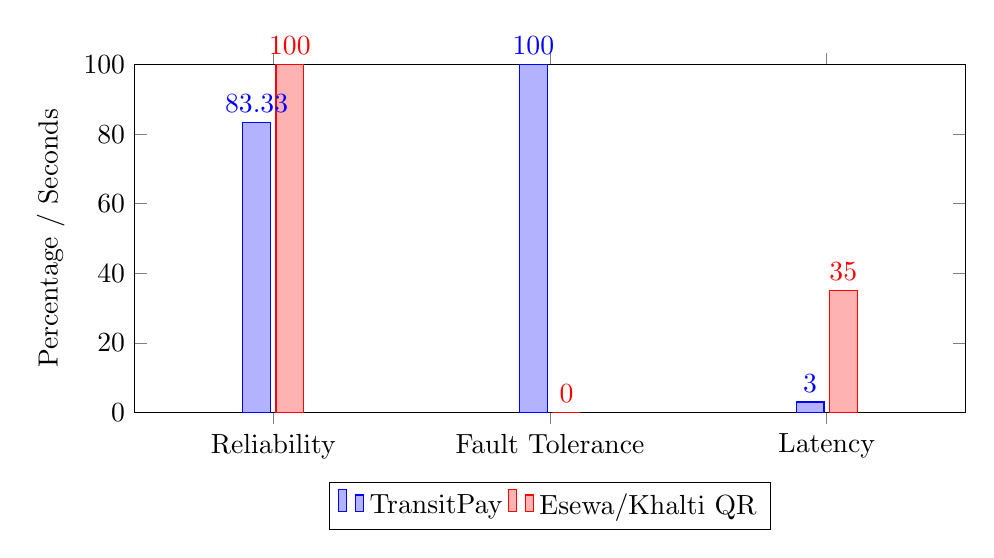
\begin{tikzpicture}
\begin{axis}[
    ybar,
    bar width=10pt,
    width=\columnwidth,
    height=6cm,
    ymin=0,
    ymax=100,
    ylabel={Percentage / Seconds},
    symbolic x coords={Reliability, Fault Tolerance, Latency},
    xtick=data,
    legend style={at={(0.5,-0.2)}, anchor=north, legend columns=-1},
    nodes near coords,
    enlarge x limits=0.25
]

\addplot coordinates {(Reliability,83.33) (Fault Tolerance,100) (Latency,3)};
\addplot coordinates {(Reliability,100) (Fault Tolerance,0) (Latency,35)};

\legend{TransitPay, Esewa/Khalti QR}

\end{axis}
\end{tikzpicture}
\caption{Performance Comparison of TransitPay and QR-based Payments}

\end{figure}

\subsection{Alignment Between Identified Problems and Proposed Solutions}

The TransitPay ecosystem was engineered as a direct technological response to the specific pain points identified in our user survey (Section 3.2). The alignment between the reported real-world challenges and the proposed technical features is summarized through the following mappings:

\begin{itemize}
    \item \textbf{Cash Dependency and Change Inavailability:} The survey highlighted significant frustration regarding the "lack of change" during peak travel hours. TransitPay eliminates the need for physical currency by utilizing NFC-enabled smartphones or tap-to-pay smart cards, allowing for exact precision in fare settlement and removing the burden of cash management from both passengers and conductors.
    
    \item \textbf{Fare Inconsistency and Overcharging:} Users reported a lack of transparency in fare calculation. The "Fair Fare Model," integrated with NEO-6M GPS modules, automates the billing process by calculating fares between exact "Tap-In" and "Tap-Out" hubs. This eliminates human error and ensures that commuters are billed strictly according to the government-mandated fare matrix (Table~\ref{tab:fare_matrix}).
    
    \item \textbf{Discount Eligibility Verification:} One of the major hurdles identified was the difficulty in verifying student or elderly discounts in real-time. The TransitPay system handles this at the "Check-in Authentication" phase (Phase 1), where the server-side role-based access control (RBAC) automatically applies the appropriate discount profile to the user's wallet without requiring physical ID verification during the trip.
    
    \item \textbf{Crowding and Manual Latency:} The identified discomfort of manual transactions in crowded buses is addressed by the 91.7\% reduction in transaction latency. By replacing manual QR scanning or cash exchange with a sub-3-second NFC tap, the system prevents "stacking" at entry points and minimizes physical interaction, thereby improving overall boarding efficiency.
    
    \item \textbf{Network Resilience:} While traditional digital wallets struggle with "patchy broadband," TransitPay's local queuing mechanism ensures that the system provides 100\% fault tolerance (Table~\ref{tab:comparison}) by allowing offline transaction capture, bridging the "Infrastructure Gap" identified in the literature review.
\end{itemize}

This mapping confirms that our proposed solution effectively bridges the structural and behavioral gaps in Nepal’s current public transit payment landscape.
\section{Discussions}


\section{Limitations}
\subsection{Cross-platform availability of host card emulation.}

\section{Conclusion}




%%
%% The acknowledgments section is defined using the "acks" environment
%% (and NOT an unnumbered section). This ensures the proper
%% identification of the section in the article metadata, and the
%% consistent spelling of the heading.
\begin{acks}
To Sunway College Kathmandu Innovation Lab, for providing the IoT based equipments and platform like Codarambha to built an MVP.
\end{acks}

%%
%% The next two lines define the bibliography style to be used, and
%% the bibliography file.
\bibliographystyle{ACM-Reference-Format}
\bibliography{sample-base}

%%
%% If your work has an appendix, this is the place to put it.
\appendix

% \section{Research Methods}

% \subsection{Part One}

% Lorem ipsum dolor sit amet, consectetur adipiscing elit. Morbi
% malesuada, quam in pulvinar varius, metus nunc fermentum urna, id
% sollicitudin purus odio sit amet enim. Aliquam ullamcorper eu ipsum
% vel mollis. Curabitur quis dictum nisl. Phasellus vel semper risus, et
% lacinia dolor. Integer ultricies commodo sem nec semper.

% \subsection{Part Two}

% Etiam commodo feugiat nisl pulvinar pellentesque. Etiam auctor sodales
% ligula, non varius nibh pulvinar semper. Suspendisse nec lectus non
% ipsum convallis congue hendrerit vitae sapien. Donec at laoreet
% eros. Vivamus non purus placerat, scelerisque diam eu, cursus
% ante. Etiam aliquam tortor auctor efficitur mattis.

% \section{Online Resources}

% Nam id fermentum dui. Suspendisse sagittis tortor a nulla mollis, in
% pulvinar ex pretium. Sed interdum orci quis metus euismod, et sagittis
% enim maximus. Vestibulum gravida massa ut felis suscipit
% congue. Quisque mattis elit a risus ultrices commodo venenatis eget
% dui. Etiam sagittis eleifend elementum.

% Nam interdum magna at lectus dignissim, ac dignissim lorem
% rhoncus. Maecenas eu arcu ac neque placerat aliquam. Nunc pulvinar
% massa et mattis lacinia.

\end{document}
\endinput
%%
%% End of file `sample-sigconf.tex'.
